\documentclass[12pt]{article}
\title{\LaTeX}
\date{}

\title{\emph{\huge\textbf{Startup Guide \\ for \\$n^3He$ Analysis}}
}
\author{\\Latiful Kabir\\
Version:1.5
}

\usepackage{listings}
\usepackage{color}
\usepackage{hyperref}
\usepackage{graphicx}

\definecolor{dkgreen}{rgb}{0,0.6,0}
\definecolor{gray}{rgb}{0.5,0.5,0.5}
\definecolor{mauve}{rgb}{0.58,0,0.82}

\lstset{frame=tb,
  language=C,
  aboveskip=3mm,
  belowskip=3mm,
  showstringspaces=false,
  columns=flexible,
  basicstyle={\small\ttfamily},
  numbers=none,
  numberstyle=\tiny\color{gray},
  keywordstyle=\color{blue},
  commentstyle=\color{dkgreen},
  stringstyle=\color{mauve},
  breaklines=true,
  breakatwhitespace=true,
  tabsize=3
}

\begin{document}
  \maketitle
  
\newpage  
\tableofcontents
\newpage
\setcounter{tocdepth}{2}

\section{Resources}
All the startup software and manual related to $n^3He$ experiment can be found from the official git repository with detailed instruction. \\
The easiest way is to go to n3He wiki (n3he.wikispaces.com) and then click on software from the left panel.  \\
Alternatively, here is a direct \href{http://latifkabir.github.io/n3He_Soft/}{link}.\\
Any new change goes to this  git repository. You might want to clone the entire repository and pull periodically to be updated. Or you can also download the last release of only what your are interested in.  

\noindent
{\color{red} \rule{\linewidth}{1mm} }
 
\newpage
\section{Quick start on basestar}
On basestar the data is being transferred and saved to the directories: \\ \textcolor{magenta}{ /mnt/idata01/data/ } (run number: 1-23661),\\ \textcolor{magenta}{ /mnt/idata02/data/ } (run number: 23662 -31839 ),\\ \textcolor{magenta}{ /mnt/idata03/data/ } (run number: 31840- 40703),\\ \textcolor{magenta}{ /mnt/idata04/data/ } (run number:40704 -44385 ),\\ \textcolor{magenta}{ /mnt/idata05/data/ } (run number:44386 - 45999 ),\\ \textcolor{magenta}{ /mnt/idata06/data/ } (run number:46000 - )\\and the analysis library is compiled in a shared directory \textcolor{magenta}{ /home/npdg/n3He/libn3He/lib} 

So a quick start using the compiled library can be as follows from any user account:

\begin{enumerate}
  \item Add the following lines to the .bashrc file \& save it
 
\begin{lstlisting}
if [ -f /home/npdg/n3He/libn3He/bin/thisn3He.sh ]; then
       . /home/npdg/n3He/libn3He/bin/thisn3He.sh
fi
\end{lstlisting}

 \item Start a new terminal , go to  \textcolor{magenta} { /home/npdg/n3He/libn3He/analysis/ }directory \& try running sample analysis scripts from ROOT.
 \item The data browser GUI (named as n3HeData) can be opened issuing the command\textcolor{magenta}{ /home/npdg/n3He/n3HeData/n3HeData } from the terminal. Copy the binary to your home directory if you will be using the GUI frequently.
\end{enumerate}

Other user specific customization can be achieved following the instruction in the ReadMe file in the respective directory.\\
For a local version of the library and data browser please read the corresponding section.

\noindent
{\color{red} \rule{\linewidth}{1mm} }
 
\newpage
\section{Event length, dead time and file size}
The  event length set in the clean DAQ at 50 KHz sample rate is :830 . Theoretically the maximum possible value is 50KHz x 16.66 ms = 833 samples per T0 . \\
But 833 event length gives occasional overlap. So we set to 830. \\
For dirty DAQ at 100 KHz the theoretical number of samples 100KHz x 16.6666 ms = 1667 \\
But to avoid overlap we set to 1660. \\
More over the DAQ has fixed dead time(readout time) of 35 samples(with no averaging) at the end of any event. This amount of time will be missed for every event.\\
\\
Clean DAQ event length 830 with nacc=16,16 with hi resolution mode=1\\
Dirty DAQ event length 1660 with nacc=1,1 with hi resolution mode=0\\
where nacc=n,n indicates how many samples being averaged.\\
\\
Thus number of sample per event:\\
Clean DAQ: (830-35)/16=49.68 $\sim$ 50  (1 header + 49 samples)\\
Dirty DAQ: (1660-35)=1625 (1 header + 1624 samples) \\
Thus the dead time in the DAQ will be --\\
Clean DAQ : (52 - 49) x 320 micro sec = .96 milli sec\\
Dirty DAQ : (1667-1624) x 10 micro sec =0.430 milli sec\\\\
Run Length/file size calculation:\\
With 25000 T0 per run- \\
Clean DAQ file size: 25000 T0 x 50 samples x 4 Byte per sample x 48 Channels =$240 \times 10^6$ Bytes\\
Dirty DAQ file size (before process): 25000 T0 x 1625 samples x 4 Bytes per sample x 8 channels = $1300 \times 10^6$ Bytes\\
Dirty DAQ file seize (after process) : 25000 T0 x 1625 samples x 4 Bytes per sample x 2 channels = $325 \times 10^6$ Bytes\\
\noindent
{\color{red} \rule{\linewidth}{1mm} }
 
\newpage
\section{The data file structure}
48 Clean DAQ channels divided into two modules: \\
Each sample is 4 bytes(in hexdump one contiguous pair consists one sample or 4 bytes). Out of this 32 bit(4 bytes) , our data is 24 bit and remaining least significant 8 bits are channel ID. \\
\begin{figure}[htb]
\centering
% Requires \usepackage{graphicx}
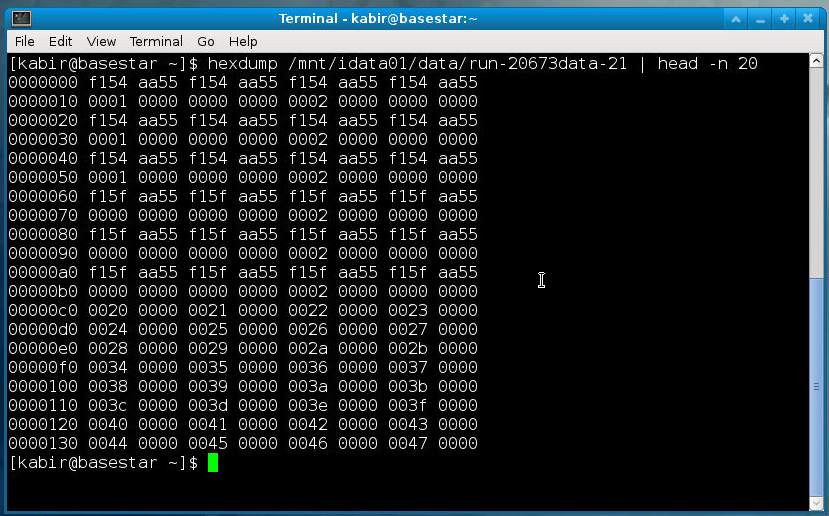
\includegraphics[width=6in]{hexdump.png}\\
\caption{Typical view of hexdump}\label{f1}
\end{figure}


The above hexdump to be interpreted as follows:\\
With: mod= module  ch = channel\\
\begingroup
    \fontsize{8pt}{12pt}\selectfont
    \begin{verbatim}      
mod1event1sample1Ch0 mod1event1sample1ch1 mod1event1sample1ch3 ..... ... ... ... ... mod1event1sample1ch8 
mod1event1sample1Ch9 mod1event1sample1ch10 mod1event1sample1ch11 ..... ... ... ... ... mod1event1sample1ch16
mod1event1sample1Ch17 mod1event1sample1ch18 mod1event1sample1ch19 ..... ... ... ... ... mod1event1sample1ch23

mod2event1sample1Ch0 mod2event1sample1ch1 mod2event1sample1ch3 ..... ... ... ... ... mod2event1sample1ch8 
mod2event1sample1Ch9 mod2event1sample1ch10 mod2event1sample1ch11 ..... ... ... ... ... mod2event1sample1ch16
mod2event1sample1Ch17 mod2event1sample1ch18 mod2event1sample1ch19 ..... ... ... ... ... mod2event1sample1ch23


mod1event2sample1Ch0 mod1event2sample1ch1 mod1event2sample1ch3 ..... ... ... ... ... mod1event2sample1ch8 
mod1event2sample1Ch9 mod1event2sample1ch10 mod1event2sample1ch11 ..... ... ... ... ... mod1event2sample1ch16
mod1event2sample1Ch17 mod1event2sample1ch18 mod1event2sample1ch19 ..... ... ... ... ... mod1event2sample1ch23

mod2event2sample1Ch0 mod2event2sample1ch1 mod2event2sample1ch3 ..... ... ... ... ... mod2event2sample1ch8
mod2event2sample1Ch9 mod2event2sample1ch10 mod2event2sample1ch11 ..... ... ... ... ... mod2event2sample1ch16
mod2event2sample1Ch17 mod2event2sample1ch18 mod2event2sample1ch19 ..... ... ... ... ... mod2event2sample1ch23
  
....     ....             ....  ...           .................             ........................    .....
....     ....             ....  ...           .................             ........................    .....
....     ....             ....  ...           .................             ........................    .....
....     ....             ....  ...           .................             ........................    .....

Up to N number of events.

\end{verbatim}    
\endgroup

Now the first sample of any event is the event header with following structure:\\
mod1event1sample1Ch0=mod1event1sample1Ch1=\\
mod1event1sample1Ch2=mod1event1sample1Ch3 = Event Signature-1 (0xaa55f154) ,\\ mod1event1sample1Ch4= Event Number\\
mod1event1sample1Ch5 = checksum using path-1  \\mod1event1sample1Ch6 = sample number \\mod1event1sample1Ch7 = checksum using path-2 \\
Then this pattern repeats 3 more times (i.e. in quanta of 8 channels) up to channel-23\\
\\
mod2event1sample1Ch0 =mod2event1sample1Ch1=mod1event1sample1Ch2 = mod2event1sample1Ch3= Event Signature-2 (0xaa55f15f) \\mod1event1sample1Ch4= 0 (always)\\
mod2event1sample1Ch5 = checksum using path-1 \\ mod2event1sample1Ch6 = sample number \\mod2event1sample1Ch7 = checksum using path-2 \\
Then this pattern repeats 3 more times (i.e. in quanta of 8 channels) up to channel-23\\
\\
For Dirty DAQ the data is taken in 8 channels (bank mask B) with one module only and then processed to 2 channels.
On Batch panel, M1 signal is connected to marked channel-26 and RFSF signal is connected to marked channel 27. This corresponds to 
ADC channel-5 (with checksum) and channel-6 (with sample number) where for ADC channel number starts with 0.\\
\\
So for the Dirty DAQ after the processing the data structure is:\\
\\
event1sample1Ch0   event1sample1ch1\\
event2sample1Ch0   event2sample1ch1\\
... ... ... ... ... ... .........\\
.....  .........  ..... .... ....\\
\\
Up to N events.\\
\\
with the first sample of any event being checksum and sample number i.e.\\
     event1sample1ch0 = checksum.\\
     event1sample1ch1 = sample number.\\

In the analysis we recommend to skip the last event to be safe in case the last event of the run is a partial event (though every effort has been made to avoid this).
     
\newpage     
\begin{figure}[htb]
\centering
% Requires \usepackage{graphicx}
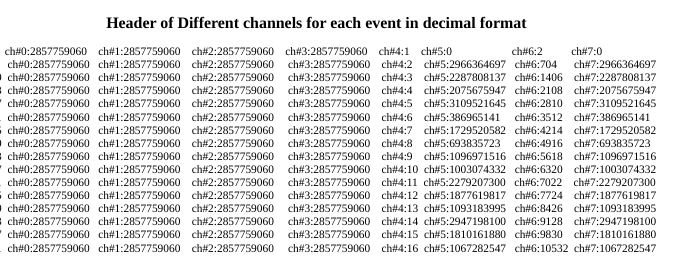
\includegraphics[width=6in]{header1.png}\\
\caption{Header of different channels for each event in decimal}\label{f1}
\end{figure}

\begin{figure}[htb]
\centering
% Requires \usepackage{graphicx}
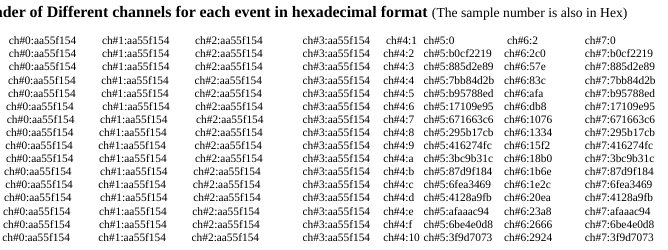
\includegraphics[width=6in]{header2.png}\\
\caption{Header of different channels for each event in hex}\label{f1}
\end{figure}

\noindent
{\color{red} \rule{\linewidth}{1mm} }
 
\newpage
\section{ADC count to Volt conversion and time bin}
The resolution and device range of a DAQ device determine the smallest
detectable change in the input signal. We can calculate the smallest
detectable change,called the precision(code width), using the following formula.
$$Precision =\frac{ADC Range}{2^{resolution}}$$
Our DAQ is a 24 bit ADC. But each sample is stored as 32 bit wording. Out of this 32 bit least significant 8 bit is the channel ID and the remaining 24 bit contains the signal. And the ADC has a range of +10 V to -10 V. Then, 
$$Precision =\frac{20 Volt}{2^{32}}$$
Thus $4.656612873\times10^{-9}$ will be an approximation for the conversion factor from ADC value to volt (if the least 8 bits are NOT thrown away). But to be precise, it is recommended to throw away the least significant 8 bit out of 32 bit, (use $ADC Count>>8$ in your analysis code), then \\
$$Precision =\frac{20 Volt}{2^{24}}$$
i.e. $1.192092896\times10^{-6}$ will be the correct ADC count to volt conversion factor(if 24 bit is used throwing away least significant 8 bit).\\

The time bin depends on the sample rate at which the DAQ is taking data. For the n3He experiment we run the clean DAQs at 50 KHz sample rate and dirty DAQs at 100KHz. Again for clean DAQs 16 samples are averaged to give one sample and for dirty DAQ no averaging is used. Thus for clean (detector) data each time bin corresponds to: 
$$16\times\frac{1}{50KHz}=320\mu sec$$
And for dirty data it is 
$$\frac{1}{100KHz} = 10 \mu sec$$

\noindent
{\color{red} \rule{\linewidth}{1mm} }
 
\newpage
\section{The ADC channel to wire map}
Out of 48 clean ADC channels, only 36 ADC channels are connected to the pre-amps (ADC channels 0 to 17 and channels 24 to 41). Moreover there are five bad channels: DAQ21- channels 5 \& 6(they are combined on channel 6), DAQ22 channels 35 and DAQ 24 channel-35,39(these have opposite polarity and can be corrected easily by flipping the sign in the analysis). \\
Following is the ADC channel to wire map for reference:
\begin{lstlisting}

Number of layers = 16;
Number of wires per layer= 9;

Layer_to_DAQ_map[Nlayers]={21, 23, 21, 23, 21, 23, 21, 23,
                         22, 24, 22, 24, 22, 24, 22, 24};

Layer_to_ADC_channel_map[16][9] =
    {
      {0,1,2,3,4,5,6,7,8},
      {0,1,2,3,4,5,6,7,8},
      {9,10,11,12,13,14,15,16,17},
      {9,10,11,12,13,14,15,16,17},
      {24,25,26,27,28,29,30,31,32},
      {24,25,26,27,28,29,30,31,32},
      {33,34,35,36,37,38,39,40,41},
      {33,34,35,36,37,38,39,40,41},
      {0,1,2,3,4,5,6,7,8},
      {0,1,2,3,4,5,6,7,8},
      {9,10,11,12,13,14,15,16,17},
      {9,10,11,12,13,14,15,16,17},
      {24,25,26,27,28,29,30,31,32},
      {24,25,26,27,28,29,30,31,32},
      {33,34,35,36,37,38,39,40,41},
      {33,34,35,36,37,38,39,40,41},
    };
\end{lstlisting}
Thus , if we label layers and wires starting from 1, then the above mapping to be interpreted as - \\
The ADC21 , channel-0 corresponds to layer 1 wire 1. \\
The ADC24, channel-40 corresponds to layer 16 wire 8.\\
The ADC22, channel-5 corresponds to layer 9 wire 6. And so on.\\  
Where (for Up-down asymmetry) wire 1 label starts from (beam) bottom of any layer. And wire 9 is the (beam) top wire of any layer.\\
And the layer counting starts from the face where beam enters the chamber. \\

\begin{figure}[htb]
\centering
% Requires \usepackage{graphicx}
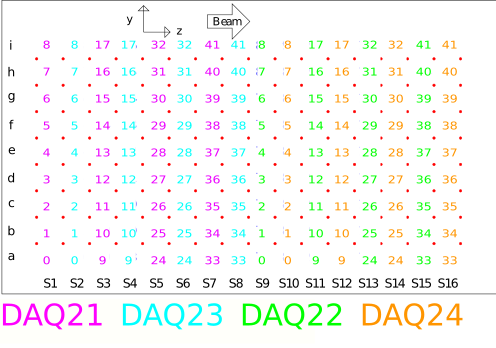
\includegraphics[width=6in]{adc2wire.png}\\
\caption{ADC to Wire Map}\label{f3}
\end{figure}


\noindent
{\color{red} \rule{\linewidth}{1mm} }
 
\newpage
\section{Setting up local version of n3He analysis library on basestar}
Eventually you will want to set up your own version of the analysis library and ROOT environment. This way you can modify any
part of the library and add more functionality. 

\begin{enumerate}
\item Download the source code from \href{http://latifkabir.github.io/n3He_Soft/}{here}. \\
lib3He is the analysis library for n3He experiment.

\item Make any necessary changes in Constants.h file that is required.

\item Do \textcolor{magenta}{ make} to compile the library. 

\item This will produce  \textcolor{magenta}{libn3He.so} (shared library will be inside lib directory).

\item Place the .so file in a directory under \textcolor{magenta}{ LD\_LIBRARY\_PATH }.

\item Now start root and load the Library as: \textcolor{magenta}{gSystem$->$Load(``libTree'')}  \& \textcolor{magenta}{gSystem$->$Load(``libn3He.so'')}  . (For Online analysis)

\item  For analysis from a script if you include TTree.h file then you need not to do \textcolor{magenta}{gSystem$->$Load(``libTree'')}; Just load 
    \textcolor{magenta}{gSystem$->$Load(``libn3He.so'')}.  You need to give full path unless the directory is included in \textcolor{magenta}{LD\_LIBRARY\_PATH}.

\item If you put the \textcolor{magenta}{rootlogon.C} file in \textcolor{magenta}{ macros } directory under Root installation directory, then the library will be loaded automatically and step-6 is NOT necessary.\\
If you do NOT have local version of ROOT, rather it's installed under root account(a shared version, which is the case for basestar by default), then just copy system.rootrc file from \textcolor{magenta}{/usr/share/root} to your home directory and rename it to \textcolor{magenta}{.rootrc}, Now add the directory having \textcolor{magenta}{rootlogon.C} file to the list of \textcolor{magenta}{Unix.*.Root.MacroPath} variable. \\
\item Now from your root script create a Tree by calling: \textcolor{magenta}{TTreeRaw ${\ast}my\_tree$ = new TreeRaw(runNumber\#)} or Just \textcolor{magenta}{TTreeRaw t(runNumber\#)}

\item Do \textcolor{magenta}{$my\_tree->Print()$} to print the tree and branch structure.

\item Now do what ever analysis you want using \textcolor{magenta}{my\_tree }.

\item Try running example analysis scripts in ``analysis" directory.

\item To make life easier it's convenient to put the following command into your \textcolor{magenta}{$\sim$/.bash\_profile} or \textcolor{magenta}{$\sim$/.bashrc} file:

 
\begin{lstlisting}
if [ -f /path/to/libn3He/bin/thisn3He.sh ]; then 
        . /path/to/libn3He/bin/thisn3He.sh
 fi 
\end{lstlisting}

Note: This version of the library works both for ROOT 5 and ROOT 6.

\end{enumerate}

\noindent
{\color{red} \rule{\linewidth}{1mm} }
 
\newpage
\section{Setting up local version of data browser on basestar}
\begin{enumerate}
\item Download the source code from \href{http://latifkabir.github.io/n3He_Soft/}{here}. \\

\item In bin directory: contains just binary files(obtained after doing make) named \textcolor{magenta}{n3HeData}.

\item In libn3He directory: Contains all the library required for running the Data check GUI.

\item Modify and compile the library (Unless you have already set up the library):
   You need to change the Data file directory from \textcolor{magenta}{Constants.h} in \textcolor{magenta}{libn3He} to appropriate directory. Before you do \textcolor{magenta}{make} do: \textcolor{magenta}{make clean}   
   in the same directory.  and then make a fresh shared binary files after you make any changes.

\item Place .so file under \textcolor{magenta}{LD\_LIBRARY\_PATH}:
   Now make sure the shared library (\textcolor{magenta}{libn3He.so}) file is in a directory under your \textcolor{magenta}{LD\_LIBRARY\_PATH}. \\ 

  Alternatively, more convenient and  professional way is as follows:
   
 Include command in your \textcolor{magenta}{.bashrc} file to run \textcolor{magenta}{thisn3He.sh} file each time you open the terminal. i.e. include the following lines:

\begin{lstlisting}
if [ -f path_to/libn3He/bin/thisn3He.sh ]; then
	. path_to/libn3He/bin/thisn3He.sh
fi
\end{lstlisting}

\item Produce binary for GUI:
To produce a new binary file named \textcolor{magenta}{n3HeData}, go to n3HeData directory, open makefile and change \textcolor{magenta}{LIB\_INCLUDE} and \textcolor{magenta}{GLIBS} to
  appropriate location for you and then do \textcolor{magenta}{make}. It will produce \textcolor{magenta}{n3HeData} binary file in the same directory. 

\item Run the GUI:
Now run the binary file \textcolor{magenta}{n3HeData} by doing \textcolor{magenta}{./n3HeData} from your recently compiled verson in \textcolor{magenta}{n3HeData/} .

\item Modify the \textcolor{magenta}{.desktop} file (included one only for Ubuntu distribution) and \textcolor{magenta}{.sh} file in bin directory accordingly and place it in your desktop if you want to run the GUI just by double clicking from your desktop.

\end{enumerate}

\begin{figure}[htb]
\centering
% Requires \usepackage{graphicx}
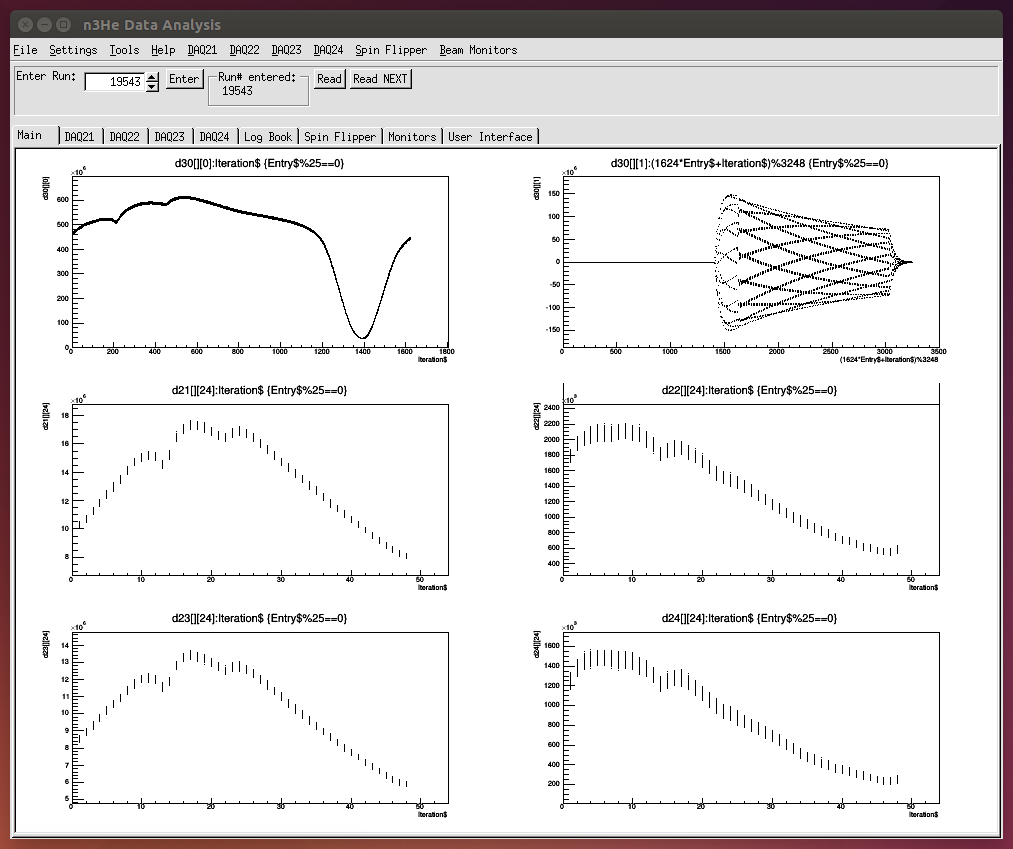
\includegraphics[width=6in]{data_browser.png}\\
\caption{The n3He data browser}\label{f2}
\end{figure}

\noindent
{\color{red} \rule{\linewidth}{1mm} }
 
\newpage
\section{Current tree structure in n3He analysis libary}

Currently n3He Tree has five branches corresponding to four clean DAQ and one dirty DAQ, following is the leaf list in the n3He Tree. 
\begin{lstlisting}
 DAQ21_LEAF "h21[48]/I:d21[49][48]/I"
 DAQ22_LEAF "h22[48]/I:d22[49][48]/I"
 DAQ23_LEAF "h23[48]/I:d23[49][48]/I"
 DAQ24_LEAF "h24[48]/I:d24[49][48]/I"
 DAQ30_LEAF "h30[2]/I:d30[1624][2]/I"
\end{lstlisting}
where h used to indicate header and d used to indicate detector signal. 21 to 24 are clean DAQs and 30 is dirty DAQ. Clean DAQs contain detector signals. Dirty DAQ (after data processing) ADC channel-0 is monitor-1 signal and ACD channel-1 is RFSF signal. 

\begin{figure}[htb]
\centering
% Requires \usepackage{graphicx}
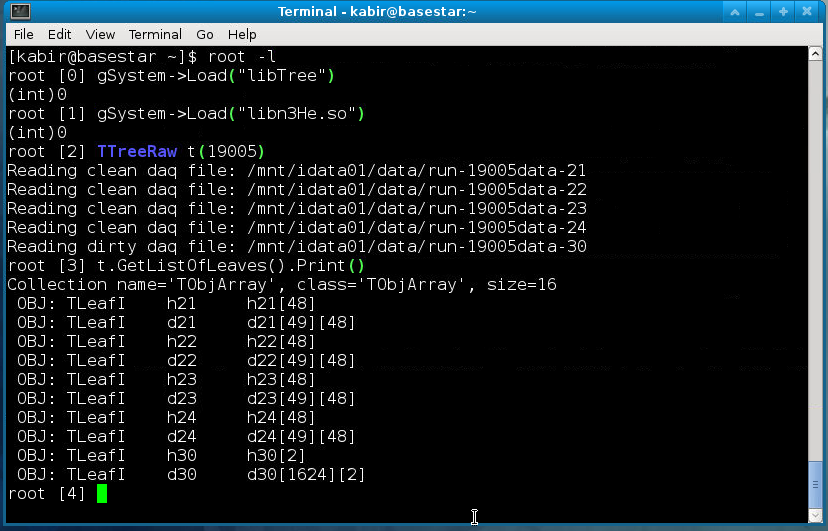
\includegraphics[width=6in]{treeStructure1.png}\\
\caption{The n3He leaf list}\label{f3}
\end{figure}

Now the library always skips the first four or five events since those might NOT be reliable. As a result the number of events in any branch for a typical n3He run is 24996 or 24995(This offset is set dynamically).Also in the analysis we recommend to skip the last event to be safe in case the last event of the run is a partial event (though every effort has been made to avoid this).


\begin{figure}[htb]
\centering
% Requires \usepackage{graphicx}
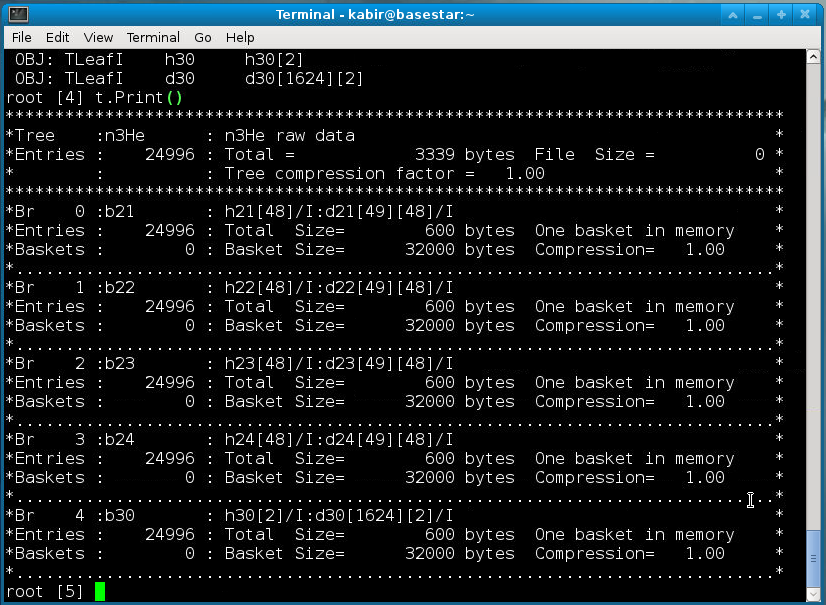
\includegraphics[width=6in]{treeStructure2.png}\\
\caption{The n3He tree structure}\label{f4}
\end{figure}

\noindent
{\color{red} \rule{\linewidth}{1mm} }
 
\newpage
\section{Sample analysis}
Sample online analysis on basestar:
\begin{lstlisting}
//OnlineAnalysis.C
//Demo Online Analysis using n3He Library.(By Online I mean  'from CINT, doing analysis on the fly, less thoughtful but preferred in some conditions')
//Author: Latiful Kabir
//Date: 12/23/14

void OnlineAnalysis()
{
    gSystem->Load("libTree");    //You need to load libTree first in order to Load libn3He. This is not necessary if you include TTree.h
    gSystem->Load("libn3He.so");

    TTreeRaw *t=new TTreeRaw(19900);
    t->Draw("d21[][0]:Iteration$");
}

\end{lstlisting}

This script when you run using \textcolor{magenta}{root -l OnlineAnalysis.C} will produce the following output:

\begin{figure}[htb]
\centering
% Requires \usepackage{graphicx}
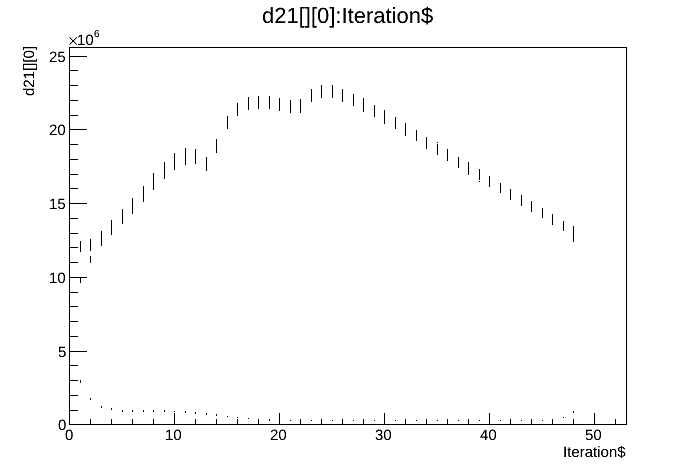
\includegraphics[width=6in]{OnlineAnalysis.png}\\
\caption{The Output from OnlineAnalysis.C}\label{f5}
\end{figure}

\newpage

Sample offline analysis on basestar:
\begin{lstlisting}
//OfflineAnalysis.C
//Demo Offline Analysis using n3He Library.(By Offline I mean  'in a script more thoughtful and serious analysis unlike from CINT)
//This script shows how to accress Tree using SetAddress
// and plots only the all event/pulses of channel-0
//Author: Latiful Kabir
//Date: 01/14/15
//This is the fastest and most preferred method for reading Tree 

#include<TTree.h>
#include<TBranch.h>
#include<TGraph.h>

void OfflineAnalysis(){

    //Load the library unless loaded automatically by ROOT
     gSystem->Load("libTree");
     gSystem->Load("libn3He.so");
 
  //Create a TTreeRaw object with desired run number
  TTreeRaw *t=new TTreeRaw(17900);
  t->Print();  // Print to see what's inside the Tree
  int ch=0; //Channel to analyze

  //Create a struc buffer to keep your events 
  struct myData
  {
      int header[48];
      int det[49][48];  
  };

  myData md;
  
  //Get the branch you want to analyze
  TBranch *b=t->GetBranch("b21");
  b->SetAddress(&md.header[0]);

//--------------------------------------------------

  TGraph *g=new TGraph();

  //Loop through all the events in the run.
  for(int i = 0;i < b->GetEntries();i++)
  {
      //Load the samples for a event/pulse in buffer
      b->GetEntry(i);

      //Loops through the sample for the loaded event
      for(int k=0;k<49;k++)
 	  g->SetPoint(i*49+k,i*49+k,md.det[k][ch]);
  }

  g->Draw("AP");
  delete t;
}
\end{lstlisting}


This script when you run using \textcolor{magenta}{root -l OfflineAnalysis.C} will produce the following output when zoomed in:

\begin{figure}[htb]
\centering
% Requires \usepackage{graphicx}
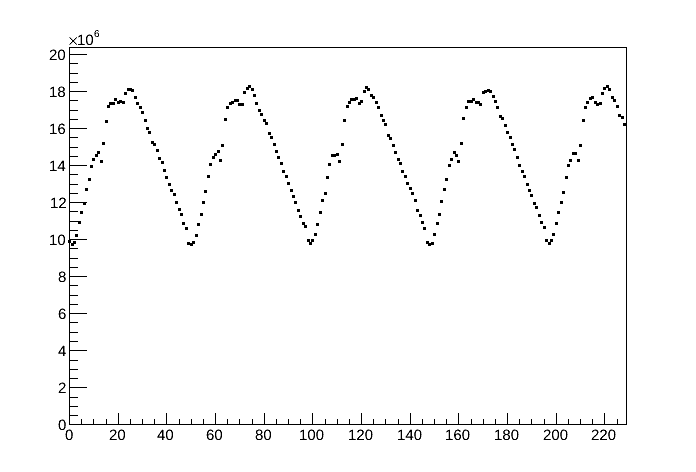
\includegraphics[width=6in]{OfflineAnalysis.png}\\
\caption{The output from OfflineAnalysis.C}\label{f6}
\end{figure}

\noindent
{\color{red} \rule{\linewidth}{1mm} }
 
\newpage
\section{Reference for TTreeRaw class}
The base Class is  TTree.\\
As a result all data and member functions from TTree are automatically inherited. For a list of TTree data and member functions go \href{https://root.cern.ch/root/html/TTree.html}{here}
\begin{lstlisting}
public:

   TString dataPath;
   TString *DaqLeaf;
   TString *dataFile;
   static int module[5];

   TBranch *b21,*b22,*b23,*b24,*b30;

   void Init(int runNumber);
   TTreeRaw(int runNumber);
   ~TTreeRaw();

\end{lstlisting}
This list will be updated gradually as new functionality is added to the TTreeRaw class.

\noindent
{\color{red} \rule{\linewidth}{1mm} }

\newpage
\section{Reference for Run numbers}
Actual n3He data with full run length(25000 T0 per run) starts from 14586. \\

Left Right(PC) Asymmetry Data : Run numbers with beam before 16390 (exclude chopper tuning, polarimetry, beam scan, collimation data runs)\\

Run range used so far for PC asymmetry analysis :14785 - 15785  \\

Chopper Tuning Data : 15867 - 15924 \\

Instrumental Asymmetry Data : 17357 - 17889 , ... ... \\

U/D Asymmetry Data : Starts from run number 17400 and continues as we take data. \textbf {For the Up-Down analysis it is recommended to use run numbers after 18000 since we were still testing and changing things before that.}\\

The stable optimization of n3He library was done for run numbers starting from 17400. \\
  
Polarimetry Data : Consecutive short runs are generally polarimetry data. Its generally taken on Wednesday of first week of the month\\

850KW and 1.2MW runs: Runs before April 25 are 850KW and after that are 1.2MW.\\

Second Collimation scan runs: 37987-38022 \\
 
\textbf{ Note: This list is NOT complete. For a complete list or reference work out through the paper log book.} \\

\noindent
{\color{red} \rule{\linewidth}{1mm} }

\newpage
\section{Summary of 1st Beam Cycle Data}
Run Range: 17400 to 38214 (excluding initial test runs)\\
Total Runs on tape(on basestar) : 20815 \\
Number of GOOD Runs :16684 \\
Number of runs with partial last event :246 (Still GOOD if last event is skipped)\\
Number of runs with header/trigger issue : 201 \\
Number of runs with partial beam or NO beam :2820 \\
Number of short runs : 802 \\
Number of runs with synchronization issue : 19 \\
Number of runs with NO data files on basestar: 43 \\
   
\textbf{ For a complete list of individual run status \\
check the file /mnt/idata05/summary/runList.txt on basestar.}

\noindent
{\color{red} \rule{\linewidth}{1mm} }

\newpage
\section{List of n3He Parameters}
Chopper 1 Phase : 14.045 CW \\
Chopper 2 Phase : 0.245 CCW \\
T0 Delay :13.5 ms \\
DAQ dead time : 0.96 ms \\
Distance between moderator and detector front face : 18 m (approx) \\
Vertical B-field(Guide field) value : -9.14$\pm$ 0.02 Gauss.\\
Number of time bin per event for detector data : 49\\
Number of time bin per event for M1 data : 1624\\
Width of each detector data time bin : 320 $\mu$ sec.\\
Width of each M1 data time bin : 10 $\mu$ sec\\
Each run length : \\
\hspace{5cm} 25000 T0 (events) (in raw file)\\
\hspace{5cm} 24996 $\pm$ 1 T0 (events) (when loaded in TTreeRaw)\\


Others to be included gradually ... ... ... \\



\noindent
{\color{red} \rule{\linewidth}{1mm} }

\end{document}
